\section{Dataset Description}
\label{sec:description}
The dataset is one workbook with seven sheets. The \emph{Master Dataset} has one row per match, so 32 rows and 58 columns. The \emph{2025 Scorecard Detail} sheet has 19 rows and 53 columns. For each side it lists the playing eleven, the coach, the batting and bowling figures, the fall of wickets, the extras split into byes, leg byes, wides and no balls, and the fours and sixes. We added boundary runs and run rate to this sheet. Team Records, Tournament Summary, Venue Analysis and Player of the Match are summaries that recalculate from the master table, and a README sheet lists notes and known gaps.

Table~\ref{tab:fields} groups the 58 fields. \emph{Team~1 always means the side that batted first.} Dates are real dates, lengths are in metres and wind speed is in kilometres per hour. Table~\ref{tab:summary} gives a picture of the two tournaments. Of the 32 matches, 20 were played at Dubai, 8 at Abu Dhabi and 4 at Sharjah, and only Dubai hosted matches in both years.

\begin{table}[!t]
\caption{Summary of the two tournaments}
\label{tab:summary}
\centering
\footnotesize
\begin{tabular}{@{}lcc@{}}
\toprule
 & \textbf{2022} & \textbf{2025} \\
\midrule
Teams and matches & 6 and 13 & 8 and 19 \\
Champion & Sri Lanka & India \\
Runner up & Pakistan & Pakistan \\
Average runs per match & 301.2 & 289.8 \\
Highest and lowest team score & 212 and 38 & 202 and 57 \\
Won by chasing and batting first side & 9 and 4 & 10 and 8 \\
Decided by Super Over & 0 & 1 \\
\bottomrule
\end{tabular}
\end{table}


Figure~\ref{fig:completeness} shows how complete each group of fields is. Identity, teams, scores, results and pitch notes are complete for both years. Weather is complete for 2022 but only about 2842\% filled for 2025. The Abu Dhabi boundary lengths and the 2025 reserve umpire are missing. We leave these gaps visible because an empty cell is easier to handle than a number that was made up.

\begin{figure}[!t]
\centering
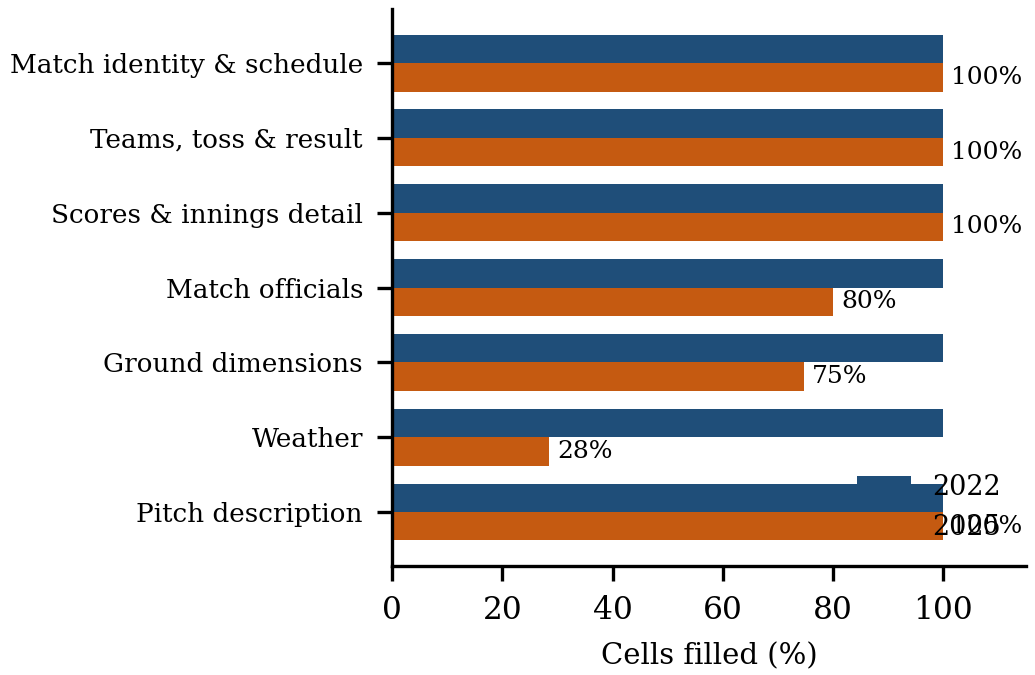
\includegraphics[width=\columnwidth]{fig_completeness.png}
\caption{Share of cells filled in, by group of fields. Numbers beside the orange bars are for 2025. Every 2022 group is complete.}
\label{fig:completeness}
\end{figure}

\begin{table*}[!t]
\caption{The 58 fields of the Master Dataset, grouped by purpose}
\label{tab:fields}
\centering
\footnotesize
\renewcommand{\arraystretch}{1.08}
\begin{tabular}{@{}p{0.14\textwidth}c p{0.48\textwidth}p{0.27\textwidth}@{}}
\toprule
\textbf{Group} & \textbf{No.} & \textbf{Fields} & \textbf{What they tell us} \\
\midrule
Identity and schedule & 13 & Match ID, Series, Year, Match Number, Match Label, Date, Group, Stage, Day, Time, Format, Venue, City & Which match, when and where \\
Ground size & 5 & Straight, Square and Mid Wicket Boundary Length, Wicket-to-Wicket Length, Pitch Width & Size of the playing area in metres \\
Weather and pitch & 7 & Temperature, Humidity, Condition, Wind Speed, Wind Direction, Pitch Condition, Weather \& Pitch Source & Conditions and where each note came from \\
Teams, toss, result & 7 & Team 1, Team 2, Toss Winner, Elected First, Match Winner, Player of The Match, Won by & Who played, the toss choice, who won and by how much \\
Scores & 6 & Team 1 Run, Team 2 Run, Powerplay Run Team 1 and 2, Team 1 and 2 Extras & Runs, first six overs, extras \\
Officials & 5 & Umpire 1, Umpire 2, TV Umpire, Reserved Umpire, Match Referee & Who ran the match \\
Calculated & 15 & Batting First, Batting Second, 1st and 2nd Innings Score, Match Loser, Result Type, Winner Batted, Toss Winner Won Match, Margin Type, Margin Value, Total Match Runs, Run Difference, Total Powerplay Runs, Total Extras, Fixture Key & Worked out from other fields by formula \\
\bottomrule
\end{tabular}
\end{table*}

